%% abtex2-modelo-include-comandos.tex, v-1.9.6 laurocesar
%% Copyright 2012-2016 by abnTeX2 group at http://www.abntex.net.br/ 
%%
%% This work may be distributed and/or modified under the
%% conditions of the LaTeX Project Public License, either version 1.3
%% of this license or (at your option) any later version.
%% The latest version of this license is in
%%   http://www.latex-project.org/lppl.txt
%% and version 1.3 or later is part of all distributions of LaTeX
%% version 2005/12/01 or later.
%%
%% This work has the LPPL maintenance status `maintained'.
%% 
%% The Current Maintainer of this work is the abnTeX2 team, led
%% by Lauro César Araujo. Further information are available on 
%% http://www.abntex.net.br/
%%
%% This work consists of the files abntex2-modelo-include-comandos.tex
%% and abntex2-modelo-img-marca.pdf
%%

% ---
% Este capítulo, utilizado por diferentes exemplos do abnTeX2, ilustra o uso de
% comandos do abnTeX2 e de LaTeX.
% ---
 
\chapter{Referencial Teórico}\label{referecial_teorico}

% % escrever algo entre o inicio de cada capitulo 
% - Ultimo paragrafo da introdução , irei mencionar o abordado em cada capitulo 
% - Inicio de cada seção conter uma descrição 
% - Palavras em ingles italico \texitt
Neste capitulo é abordado o referencial teórico, utilizado como embasamento para a construção deste trabalho.
% ---
\section{ Controle na Segurança Publica Brasileira }
Atualmente no Brasil existem dois sistemas informatizados utilizados por órgãos públicos para realizar a regulamentação e o monitoramento de armas de fogo, munições e demais produtos controlados.
Sendo estes, o Sistema de Gerenciamento Militar de Armas (SIGMA) e o Sistema Nacional de Armas (SINARM). O SIGMA é administrado pelo Exército Brasileiro e é responsável pelo controle de armas de fogo e munições no âmbito da Força. O SINARM é administrado pela Polícia Federal e é responsável pelo controle de armas de fogo e munições em poder da população civil \cite{shotEntendaSinarm}.

\subsection{SIGMA e SINARM}\label{sigmaesinarm}
A principal diferença entre SIGMA e SINARM é o âmbito de atuação. O SIGMA é responsável pelo controle de armas de fogo e munições no âmbito do Exército Brasileiro, enquanto o SINARM é responsável pelo controle de armas de fogo e munições em poder da população civil.
Outra diferença entre os dois sistemas é a natureza das informações que eles gerenciam. O SIGMA gerencia informações sobre armas de fogo e munições de uso militar, enquanto o SINARM gerencia informações sobre armas de fogo e munições de uso civil.
A seguir, está uma tabela comparativa que resume as principais diferenças entre ambos: 
\begin{table}[ht]
	\centering
	\caption{Comparação entre SIGMA e SINARM}
	\begin{tabularx}{\textwidth}{lXp{5cm}}
	  \toprule
	  Característica & SIGMA & SINARM \\
	  \midrule
	  Âmbito de atuação & Exército Brasileiro & População civil \\
	  Natureza das informações & Armas de fogo e munições de uso militar & Armas de fogo e munições de uso civil \\
	  Responsável pela administração & Exército Brasileiro & Polícia Federal \\
	  \bottomrule
	\end{tabularx}
  \end{table}

  
% \section{Segurança Publica - Integração SIGMA e SINARM}
% \cite[Em 2019, a Polícia Federal autorizou que o Exército tenha acesso ao Sinarm, já os militares não permitiram a liberação das informações do Sigma para os agentes da PF]{sbtnewsExxE9rcitoPolxEDcia}
% \cite{inDECRETO9847}

\section{ Sistema SIGMA } 
O Sistema de Gerenciamento Militar de Armas (SIGMA) é um sistema computacional desenvolvido pelo Centro de Desenvolvimento de Sistemas (CDS) do Exército Brasileiro e  implantado em 2003 que vem sendo constantemente atualizado para atender às necessidades da força \cite{fenemeReunixE3oSobre}.

\subsection{Contexto de implantação}
O contexto da implantação do SIGMA foi a necessidade de modernizar o sistema de controle de armas de fogo e munições do Exército Brasileiro.
O SIGMA foi desenvolvido com base nas melhores práticas internacionais de controle de armas de fogo. O sistema é integrado a outros sistemas de informação do Exército Brasileiro, o que permite a troca de dados e informações entre as diferentes áreas da força \cite{fenemeReunixE3oSobre}.

\subsection{AEL}
O Arquivo Eletrônico em Lote (AEL) é um arquivo digital que contém as informações necessárias para o cadastro de produtos controlado no SIGMA.
O AEL é utilizado para o cadastro de armas de fogo de diversas entidades, como as Forças Armadas, as forças auxiliares, a Polícia Militar e o Corpo de Bombeiros \cite{ExércitoBrasileiro}.

O Objetivo do AEL no sistema SIGMA é permitir o cadastro de produtos controlados de diversas entidades de forma centralizada e organizada. O AEL é um elemento importante do SIGMA, pois permite que o Exército Brasileiro tenha um controle mais eficiente das armas de fogo em circulação no país \cite{ExércitoBrasileiro}.

\subsection{Arquivo AEL na Brigada Militar do Rio Grande do Sul}
O AEL no contexto da BM RS, deve ser gerado para o cadastro de armas de fogo de policiais militares. O arquivo deve conter as seguintes informações:
\begin{itemize}
    \item Identificação da Brigada Militar: número do QG, código da OM e nome da OM.
    \item Identificação do armamento: número da arma, tipo de arma, marca, modelo, calibre e série.
    \item Identificação do proprietário: nome completo, CPF, RG, endereço e telefone.
    \item Além das demais informações especificadas nos anexos \ref{sec:anexoA2} e \ref{sec:anexoA3}.
\end{itemize}


O AEL deve ser gerado em um formato texto, seguindo um layout pré-definido e estar conforme os parâmetros de indexação das informações constantes nos anexos \ref{sec:anexoA1} e \ref{sec:anexoA4}.

\section{Gerenciamento de processos}
É uma abordagem disciplinada e sistemática que envolve práticas relacionadas aos processos de negócio, automatizados ou não, com o objetivo de alcançar resultados consistentes e alinhados com as metas estratégicas de uma organização. 
Conforme \citeonline{davila2008inovaccao} ``As organizações tentam inovar para se diferenciar e obter vantagens competitivas, tanto pela melhoria nos bens/serviços fornecidos quanto pela eficiência operativa''.
 Pode-se concluir que os sistemas de informação oferecem inúmeros benefícios para uma organização, sejam eles para melhorar o fluxo de informação, as tomadas de decisões, o controle de qualidade, ou ampliar a produtividade.
\subsection{BPMN}
O modelo e notação de processos de negócios (\textit{Business Process Model and Notation}) é uma notação gráfica padronizada para desenhar processos de negócios em um fluxograma. A diagramação BPMN é intuitiva e permite a representação de detalhes complexos do processo. A simbologia deste modelo serve como uma linguagem padrão, colocando um fim na lacuna de comunicação entre a modelagem do processo e sua execução, para \citeonline{bitencourt2016elicitaccao}:
\begin{citacao}
	
	Modelo de processos de negócio representa os processos de negócio de uma empresa e permite a documentação, simulação, compartilhamento, implementação, avaliação e melhoramento continuo das operações, com o intuito de compreender o funcionamento da organização e os aspectos do seu domínio \cite{bitencourt2016elicitaccao}.
	
\end{citacao}
Em resumo, o levantamento e registro da situação atual dos processos, seguido por uma análise aprofundada, são práticas essenciais para promover a eficiência, a eficácia e a adaptação contínua dentro de uma organização. Essa abordagem sistemática para entender e aprimorar os processos é fundamental para a sustentabilidade organizacional.

\section{Padrões de Projeto de Sistemas}
Padrões de desenvolvimento de software referem-se a soluções reutilizáveis para problemas comuns encontrados no processo de desenvolvimento de software. Esses padrões são abstrações que encapsulam as melhores práticas, representando soluções testadas e comprovadas para desafios recorrentes. Eles fornecem diretrizes para o design e implementação de código, promovendo a consistência, a manutenibilidade e a eficiência no desenvolvimento de software \cite{padroesProjeto}.

O contexto dos padrões de desenvolvimento de software está relacionado aos desafios enfrentados pelos desenvolvedores ao criar sistemas de software complexos. Conforme abordado por \citeonline{padroesProjeto} ``Um padrão de projeto nomeia, abstrai e identifica aspectos problemáticos comuns e propõe uma solução padrão para esses problemas''.


\subsection{Arquitetura Cliente Servidor}
Nessa arquitetura, o software é dividido em duas partes principais: o cliente e o servidor.

O cliente é a parte do sistema que interage diretamente com o usuário. Ele envia solicitações de serviço ao servidor e exibe os resultados recebidos ao usuário. O cliente pode ser um aplicativo de desktop, um aplicativo móvel ou um navegador da web, dependendo do tipo de sistema que está sendo desenvolvido \cite{flanagan2012javascript}.

O servidor é responsável por processar as solicitações recebidas do cliente e fornecer os recursos ou serviços solicitados. Ele possui os recursos necessários para atender às solicitações, como bancos de dados, aplicativos e serviços web. O servidor está sempre ativo, aguardando solicitações dos clientes e respondendo a elas de maneira apropriada \cite{arqClientServer2}.

A comunicação entre o cliente e o servidor ocorre por meio de uma rede, geralmente a Internet. O cliente envia uma solicitação para o servidor, especificando o tipo de serviço desejado e quaisquer parâmetros necessários.
Então de acordo com \citeonline{arqClientServer2}.
\begin{citacao}
O servidor, quando recebe a mensagem, extrai os parâmetros 
e chama o procedimento especificado na mensagem. No fim da execução do procedimento é 
realizada a operação inversa, colocando os resultados e enviando a mensagem de resposta ao 
processo cliente \cite{arqClientServer2}.
\end{citacao}

    Logo uma das principais vantagens da arquitetura cliente-servidor é a divisão clara de responsabilidades entre ambos. 
O cliente lida com a interface do usuário e a apresentação dos dados, enquanto o servidor cuida do processamento das solicitações e do acesso aos recursos. Isso permite uma melhor organização do sistema e facilita a manutenção e a escalabilidade.
Além disso, a arquitetura cliente-servidor permite que vários clientes acessem o mesmo servidor simultaneamente. Isso possibilita o compartilhamento de recursos e serviços, o que é especialmente útil em ambientes corporativos \cite{arqClientServer2}.

A \autoref{fig:grafico-client-server} demonstra a maneira como ocorre essa comunicação:

\begin{figure}[htb]
    \caption{\label{fig:grafico-client-server}Arquitetura Cliente-Servidor}
    \begin{center}
        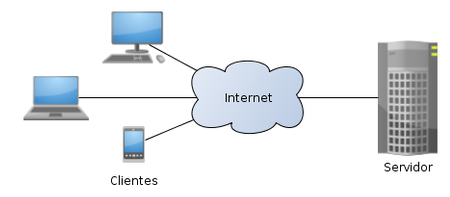
\includegraphics[scale=0.9]{imagens/arquitetura-cliente-servidor.png}
    \end{center}
    \legend{Fonte: \citeonline{Redes}}
\end{figure}


\subsection{Arquitetura MVC}
A arquitetura MVC \textit{Model-View-Controller} é um padrão de design que organiza o código de uma aplicação em três componentes principais: \textit{Model} (Modelo), \textit{View} (Visão) e \textit{Controller} (Controlador). Cada componente tem uma responsabilidade específica na aplicação, o que ajuda a manter o código modular, escalável e de fácil manutenção \cite{engsoftmoderna}.

\begin{itemize}
    \item Visão: Lida com a apresentação dos dados ao usuário e interage com o Modelo. A Visão exibe as informações e envia eventos do usuário para o Controlador.
    \item Controlador: Recebe entradas do usuário, processa essas entradas (geralmente envolvendo o Modelo) e atualiza a Visão. O Controlador age como um intermediário entre o Modelo e a Visão.
    \item Modelo: Representa a lógica de negócios e os dados da aplicação. Geralmente, o modelo é responsável pela interação com o banco de dados e pela manipulação dos dados.
\end{itemize}
Conforme exemplificado o fluxo da arquitetura MVC na \autoref{fig:grafico-mvc}

\begin{figure}[htb]
    \caption{\label{fig:grafico-mvc}Arquitetura MVC}
    \begin{center}
        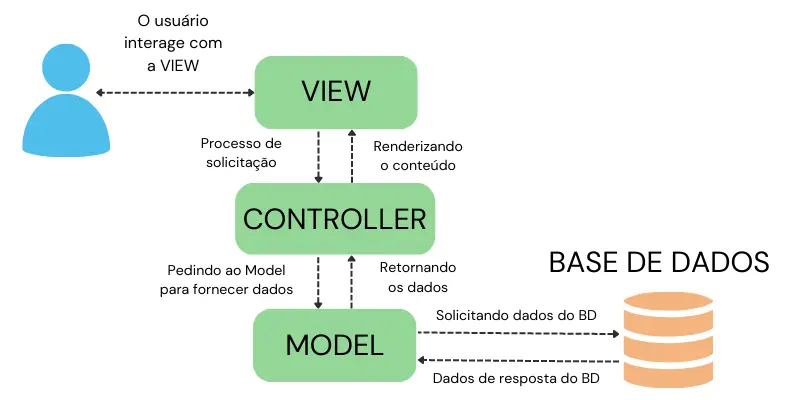
\includegraphics[scale=0.7]{imagens/arquitetura-mvc.png}
    \end{center}
    \legend{Fonte: \citeonline{engsoftmoderna}}
\end{figure}


\section{Aplicações Web}
Aplicações web são programas que são executados em navegadores e são acessados por meio de internet.
Surgiram na década de 1990 e se tornaram populares por permitirem a interação do usuário e o processamento de dados.

Existem dois tipos principais: estáticas (HTML, CSS e JavaScript) e dinâmicas (linguagens de programação do lado do servidor).
De acordo com \citeonline{aplicacoesWeb} as aplicações estáticas geralmente consistem em páginas web com conteúdo fixo, sem interação avançada ou processamento de dados em tempo real. O navegador do cliente solicita páginas estáticas ao servidor, que retorna arquivos HTML, CSS e JavaScript. A renderização e interação ocorrem no navegador.

Aplicações Dinâmicas apresentam interatividade avançada e processamento de dados em tempo real quando o navegador solicita uma página ao servidor. O servidor executa a lógica de negócios, acessa dados do banco de dados, gera dinamicamente o conteúdo HTML e o envia de volta ao navegador. Pode haver interações adicionais entre o navegador e o servidor 
oferecendo diversos benefícios como acessibilidade, atualização, redução de custos e escalabilidade \cite{aplicacoesWeb}.

\subsection{Linguagem JavaScript}
Uma linguagem de programação amplamente usada no desenvolvimento web de acordo com a organização \citeonline{mozillaJavaScript}. Ela permite adicionar interatividade e dinamismo a páginas da web. Além de ser usado no desenvolvimento de interfaces de usuário, o JavaScript também pode ser usado no desenvolvimento de aplicativos do lado do servidor (backend) com o uso de tecnologias como o Node.js. Conforme \citeonline{flanagan2012javascript} ``Javascript já deixou para trás suas raízes como linguagem de script há muito tempo, tornando-se uma linguagem de uso geral, robusta e eficiente''.

\subsection{Frameworks e Bibliotecas}
A necessidade da utilização de \textit{frameworks} surgiu com a complexidade crescente das aplicações de software.
\begin{citacao}
	Diversos \textit{frameworks} têm sido desenvolvidos nas duas últimas décadas, visando o
	reuso de software e consequentemente a melhoria da produtividade, qualidade e
	manutenibilidade \cite{maldonado2002padroes}.
\end{citacao}
Sendo estes estruturas ou conjuntos de ferramentas que fornecem uma base organizada para o desenvolvimento de aplicações. Eles oferecem uma estrutura pré-definida que acelera o processo de desenvolvimento, promove a reutilização de código e estabelece padrões de boas práticas. No contexto do desenvolvimento de software, os frameworks desempenham um papel significativo, influenciando a forma como as aplicações são projetadas, implementadas e mantidas \cite{maldonado2002padroes}.

Portanto para \citeonline[p.~23]{maldonado2002padroes} os \textit{frameworks} estão divido em dois tipos sendo eles:
\begin{itemize}
    \item Caixa preta: Uma abordagem caixa preta trata um sistema ou componente como uma entidade onde o foco está no comportamento externo, sem conhecimento detalhado de sua implementação interna, pois na maioria dos casos o desenvolvedor não tem acesso ao código fonte e a ênfase está nos resultados visíveis e nas funcionalidades oferecidas pelo sistema, sem a necessidade de compreender a lógica interna do sistema \cite[p.~23]{maldonado2002padroes}.
    \item Caixa branca: Em contraste, uma abordagem caixa branca envolve uma compreensão detalhada da implementação interna de um sistema ou componente, incluindo sua lógica, estrutura e fluxo de controle e a ênfase está na compreensão completa do sistema, possibilitando otimizações, depuração precisa e ajustes finos \cite[p.~23]{maldonado2002padroes}.
\end{itemize}

Entretanto muito semelhante aos \textit{frameworks} exceto por algumas diferenças abordados na \autoref{tab:comparacao_bibliotecas_frameworks}, existem também as bibliotecas de \textit{software} que são conjuntos de códigos preexistentes e funcionalidades encapsuladas que foram desenvolvidos para abordar tarefas comuns ao desenvolvimento de sistemas. 
Conforme \citeonline{cechinel2017avaliaccao} torna-se evidente que esses recursos desempenham um papel fundamental na eficiência e na evolução contínua do desenvolvimento de \textit{software}. Desde a reutilização inteligente de código até a adaptação às inovações tecnológicas.


\begin{table}[h]
    \centering
    \begin{tabularx}{\textwidth}{X X X}
      \toprule
      \textbf{Característica} & \textbf{Bibliotecas} & \textbf{Frameworks} \\
      \midrule
      Definição & Fornecem funcionalidades específicas. & Oferecem uma estrutura abrangente. \\
      \midrule
      Flexibilidade & Mais flexibilidade para os desenvolvedores. & Menos flexibilidade devido a maiores convenções. \\
      \midrule
      Integração & Integração opcional e modular. & Impõem uma estrutura mais integrada. \\
      \midrule
      Modularidade & Modular, escolha de partes específicas. & Estrutura monolítica, menos modularidade. \\
      \bottomrule
    \end{tabularx}
    \caption{Comparação Entre Bibliotecas e Frameworks no Desenvolvimento de Software}
    \label{tab:comparacao_bibliotecas_frameworks}
  \end{table}

\subsubsection{Node}
 Conforme o site oficial do \citeonline{Nodejs}, este é um ambiente de tempo de execução javascript que permite que o javascript seja executado no lado do servidor. Utilizando o mecanismo V8 do Google Chrome para executar código javascript fora do navegador.
 Com o Node.js, é possível criar aplicativos web e serviços \textit{backend} usando javascript. Ele fornece uma variedade de recursos e uma ampla gama de bibliotecas e frameworks, tornando-o uma escolha popular para o desenvolvimento de servidores e APIs \cite{Nodejs}.
Portanto para \citeonline{pereira2014aplicações}.
    \begin{citacao}
        Node.js é multiprotocolo, ou seja, com ele será possível trabalhar com os protocolos: HTTP, HTTPS, FTP, SSH, DNS, TCP, UDP, WebSockets e também existem outros.Toda aplicação web necessita de um servidor para disponibilizar todos os seus  recursos \cite{pereira2014aplicações}.
    \end{citacao}

Amplamente utilizado em conjunto com o node, é o framework express para aplicativos web do lado do servidor, construído sob a base nativa HTTP do Node.js.
     Ele fornece uma abordagem simplificada para lidar com solicitações HTTP, roteamento e manipulação de middleware. 
	 O Express permite criar facilmente APIs robustas e eficientes, tornando o desenvolvimento de aplicativos web mais rápido e produtivo. É um dos frameworks mais populares para o desenvolvimento de servidores com Node.js
     \cite{pereira2014aplicações}.

\subsubsection{ReactJS}
React é uma biblioteca javascript \textit{Open Source} lançado em 2013 pela \citeonline{ReactMet54}, que rapidamente ganhou popularidade devido a sua abordagem inovadora utilizada para criar interfaces de usuário. 
Através da possibilidade de escrever código utilizando a sintaxe JSX, a qual é uma convenção opcional no react que possibilita ter a organização do código javascript de maneira mais próxima à estrutura de marcação XML ou HTML.

    Logo essa biblioteca permite desenvolver componentes reutilizáveis e interativos utilizados na construção de \textit{UIS} modernas e responsivas. Possibilitando o desenvolvimento de aplicações web complexas e dinâmicas, dividindo-as em componentes reutilizáveis \citeonline{ReactMet54}.

    A partir da premissa de que a abordagem principal do React é baseada em componentes, isso facilita a criação e o gerenciamento de estado dos elementos da interface. Permitindo a criação de aplicações eficientes e escaláveis, sendo como principal característica a renderização reativa, o que faz com que a interface do usuário seja atualizada automaticamente quando o estado dos dados é alterado. Isso simplifica o desenvolvimento e melhora o desempenho, pois apenas as partes afetadas da interface são atualizadas, em vez de recarregar a página inteira \cite{ReactMet54}.

\section{Banco de dados NOSQL}
Banco de dados NoSQL é um tipo de banco de dados que difere dos bancos de dados relacionais tradicionais (SQL) em sua estrutura de armazenamento e modelo de dados. NoSQL significa \textit{Not Only SQL} (Não Apenas SQL) e abrange diversos tipos de bancos de dados que oferecem uma abordagem alternativa para o armazenamento e recuperação de dados.
Para \citeonline{pereira2014aplicações} uma das vantagens em se trabalhar com um banco de dados desse modelo é o grande suporte oferecido pela comunidade do nodejs e uma vasta gama de compatibilidade com diversas tecnologias.

Dentre as principais tecnologias que tem uma alta sinergia nesse padrão não relacional são: 


\begin{itemize}
    \item MongoDB: um eficiente e popular banco de dados NoSQL. Que utiliza um sistema de gerenciamento de banco de dados orientado a documentos, o que significa que os dados são armazenados em documentos semelhantes a JSON, em vez de tabelas com linhas e colunas como em um banco de dados relacional \cite{pereira2014aplicações}.
    Outra característica importante do MongoDB é sua capacidade de escalar horizontalmente. Oferecendo recursos avançados, como indexação, consultas poderosas e suporte a transações, tornando-o adequado para uma ampla gama de aplicações. É frequentemente utilizado em aplicativos web, análise de dados, e outras aplicações que exigem flexibilidade e escalabilidade \cite{pereira2014aplicações}.
    \item Mongoose:  Uma biblioteca ODM \textit{Object Data Modeling} para Node.js e MongoDB. Sendo inserida como uma camada de abstração facilitando a conexão, a modelagem de dados, a execução de consultas, e a interação com o banco de dados de maneira eficiente e organizada \cite{pereira2014aplicações}.

\end{itemize}


% \section{Backend}
% É a parte de um sistema ou aplicação que lida com a lógica de negócios, processamento de dados e a comunicação com o banco de dados. Envolve a criação de servidores, APIs (Application Programming Interfaces) e serviços que fornecem os dados e funcionalidades necessárias para o funcionamento do sistema. Para o desenvolvimento backend, são utilizadas diversas tecnologias, como linguagens de programação (como JavaScript, Python, Java, etc.), bancos de dados (como MySQL, PostgreSQL, MongoDB, etc.) e frameworks (como Node.js, Django, Ruby on Rails, etc.). Então o backend deve ser capaz de servir ao front-end a comunicação em tempo real entre cliente e servidor — que seja rápido, atenda muitos usuários ao mesmo tempo e utilize recursos de I/O (dispositivos de entrada ou saída) de forma eficiente ( RIBEIRO, CAIO , 2013)

% \subsection{Apis Restful}

\subsection{Segurança e autenticação}
A segurança e a autenticação em aplicações web são fundamentais para proteger dados e usuários. Utilizando criptografia,  e práticas de desenvolvimento seguro, é possível mitigar riscos, garantindo a integridade e confiabilidade do sistema. Estratégias como autenticação por token e hashing de senhas fortalecem a proteção, assegurando uma navegação online para o usuário segura e confiável \cite{segurancaeauth}.

\begin{itemize}
    \item Passport-Local: De acordo com o site oficial do \cite{passport84}, este é uma estratégia de autenticação fornecida pelo Passport.js para autenticar usuários usando um nome de usuário e senha em aplicativos Node.js. Ele é facilmente integrado a qualquer aplicativo ou framework que suporte middlewares do estilo \textit{Connect}, incluindo o Express. O Passport-local requer um retorno de chamada de verificação que valida as credenciais do usuário. Ele pode ser configurado para realizar a autenticação localmente, verificando o nome de usuário e a senha no banco de dados da aplicação. 
    \item Token JWT: \textit{JSON Web Token} (JWT) fornece uma abordagem segura para a troca de informações entre cliente e servidor por meio de um token gerado o qual tem como resultado final um objeto JSON, conforme explicado por Lucas, Ana e Jackson.
    \begin{citacao}
        O token gerado pelo JWT é salvo
        no dispositivo do usuário e suas informações podem ser verificadas a cada solicitação,
        pois são criptografadas utilizando um segredo, através do algoritmo \textit{HMAC} ou de um par de chaves públicas e privadas, garantindo assim a sua confiabilidade \cite{segurancaeauth}.
    \end{citacao}
    A \autoref{fig:grafico-jwt} exemplifica o fluxo de autenticação por token jwt: 

\begin{figure}
    \caption{\label{fig:grafico-jwt} Fluxo de autenticação JWT}
    \begin{center}
        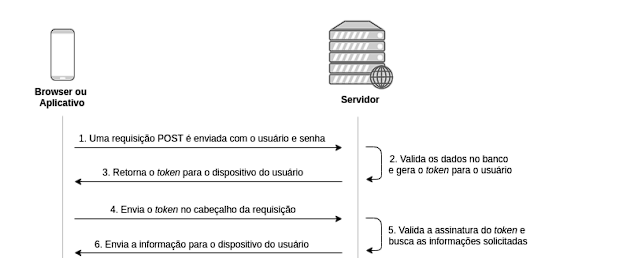
\includegraphics[scale=0.9]{imagens/jwt.png}
    \end{center}
    \legend{Fonte: \citeonline{segurancaeauth}}
\end{figure}
    
\end{itemize}

% \section{Frontend}
% É a parte de um sistema ou aplicação que os usuários interagem diretamente. Envolve a criação da interface do usuário, a implementação de elementos visuais, como layout, design, botões, formulários, etc., e a interação com o usuário por meio de eventos e ações. Para o desenvolvimento front-end, são utilizadas tecnologias como HTML (Hypertext Markup Language), CSS (Cascading Style Sheets) e JavaScript. Todo o HTML e o CSS que escrevemos ganha vida dentro dos navegadores utilizados por quem acessa nossas páginas e sites (MAZZA LUCAS, 2012)

% \begin{itemize}
%     \item HTML: (HyperText Markup Language) é a linguagem de marcação usada para estruturar e exibir o conteúdo de uma página da web. Ele fornece uma estrutura básica para a criação de elementos, como cabeçalhos, parágrafos, listas, links e imagens. O HTML é a espinha dorsal de qualquer página da web e é complementado por CSS e JavaScript para fornecer estilos e interatividade.
%     \item CSS: CSS (Cascading Style Sheets) é uma linguagem usada para estilizar a aparência dos elementos em uma página da web. Ele permite controlar cores, fontes, margens, posicionamento e outros aspectos visuais dos elementos HTML. O CSS é usado em conjunto com o HTML para criar layouts atraentes e responsivos. Ele oferece flexibilidade para personalizar o estilo de um site e torná-lo visualmente agradável para os usuários. 


% \end{itemize}
 

